\documentclass[10pt]{beamer}

\usetheme{metropolis} % Theme source: github.com/matze/mtheme
\usepackage{appendixnumberbeamer}

\usepackage{booktabs}
\usepackage[scale=2]{ccicons}

\usepackage{xspace}
\newcommand{\themename}{\textbf{\textsc{metropolis}}\xspace}

\usepackage{caption}
\setbeamertemplate{caption}[numbered]
\captionsetup{justification=centering, singlelinecheck=false}

\title{Exploring AI Agent Systems and Orchestration}
\subtitle{Directed Studies}
\author{Natalie Lambert}
\date{August 14, 2026}

\begin{document}

\maketitle

\begin{frame}{Outline}
	\begin{itemize}
		\item Introduction
		\item Agent Architectures
		\item Workflow Coordination
		\item Context Management
		\item Measuring and Evaluating Agents
		\item Discussion and Future Work
		\item Conclusion
	\end{itemize}
\end{frame}

\section{Introduction}

\begin{frame}[fragile]{Background and Motivation}
	\begin{itemize}
		\item AI agent systems have emerged as a new way to integrate vanilla LLMs into composite systems
		\item In this directed studies, I treated LLMs as blackboxes, and examined how AI agents
			can be reasoned about from a systems perspective
		\item As LLM capabilities plateau, researchers examine ways that agent systems can surpass
			basic LLM performance
	\end{itemize}
\end{frame}

\section{Agent Architectures}
\begin{frame}{Single Agent Systems}
  \begin{columns}[T,onlytextwidth]
    \begin{column}{0.5\textwidth}
	  \begin{figure}
		\centering
		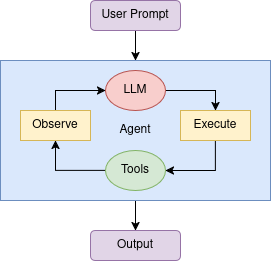
\includegraphics[width=0.75\textwidth]{figures/SAS.png}
		\caption{Most single-agent systems follow the Reason and Act (ReAct) paradigm.}
	  \end{figure}
	\end{column}
    \begin{column}{0.5\textwidth}
		\begin{itemize}
			\item Comprised of an LLM, a tool call interface and an iterative harness
			\item Well-suited for tasks that allow for linear reasoning
			\item Most effective if using a frontier LLM
		\end{itemize}
	\end{column}
  \end{columns}
\end{frame}

\begin{frame}{Multi-Agent Systems}
  \begin{columns}[T,onlytextwidth]
    \begin{column}{0.5\textwidth}
	  \begin{figure}
        \centering
        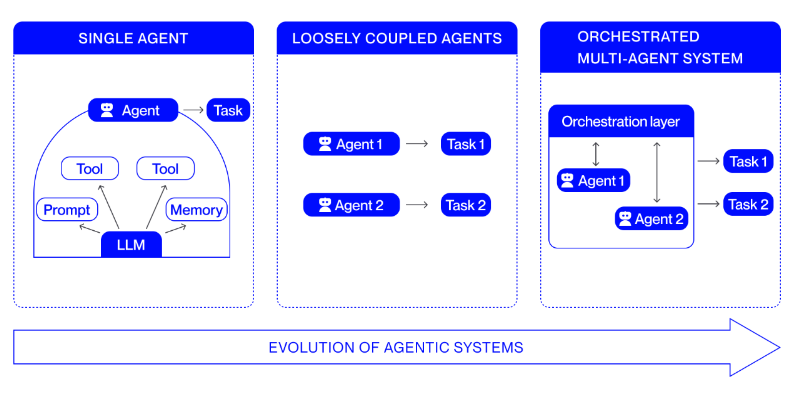
\includegraphics[width=1.0\textwidth]{figures/agent_evolution.png}
		\caption{Agent systems have evolved to into more complicated interactions between single agents
		  \href{arxiv.org/abs/2601.13671}{(\underline{source})}.}
      \end{figure}
	\end{column}
    \begin{column}{0.5\textwidth}
      \begin{itemize}
		\item A group of individual agents working in tandem on a task
		\item Can support non-linear and parallel reasoning sequences
		\item Depending on the workflow, inter-agent communication may be a bottleneck
	  \end{itemize}
	\end{column}
  \end{columns}
\end{frame}

\begin{frame}{Using Both: Cascade and Routing Strategies}
  \begin{columns}[T,onlytextwidth]
	\begin{column}{0.5\textwidth}
	  \begin{figure}
		\centering
		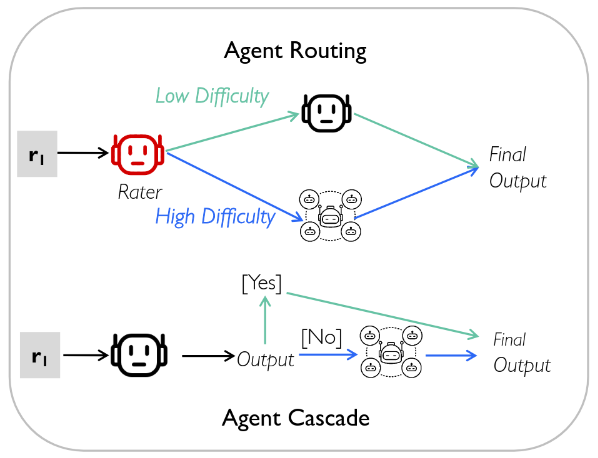
\includegraphics[width=1.0\textwidth]{figures/mas-routing.png}
		\caption{Schematic comparing cascade and routing between an SLM and LLM
		  \href{arxiv.org/abs/2505.18286}{(\underline{source})}.}
	  \end{figure}
	\end{column}
    \begin{column}{0.5\textwidth}
	  \begin{itemize}
	    \item So-called ``hybrid'' systems
		\item Routing: an LLM-as-judge determines a complexity score for a task, and
			assigns the task to a MAS (high complexity) or to a SAS (low complexity)
		\item Cascade: an SAS first attempts to solve a task; upon
			failure, the task is redirected to a MAS
	  \end{itemize}
	\end{column}
  \end{columns}
\end{frame}

\section{Workflow Coordination}

\begin{frame}{Independent Multi-Agent Systems}
  \begin{columns}[T,onlytextwidth]
    \begin{column}{0.5\textwidth}
	  \begin{figure}
		\centering
		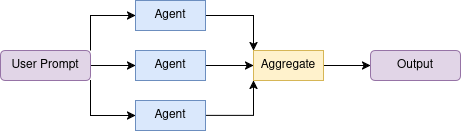
\includegraphics[width=1.0\textwidth]{figures/mas-indep.png}
		\caption{Three agents solve the same task in parallel, and all the outputs are aggregated
		for a final response.}
	  \end{figure}
	\end{column}
    \begin{column}{0.5\textwidth}
	  \begin{itemize}
		\item Multiple non-communicating agents solve tasks in parallel,
			after which all the outputs are aggregated
		\item Best used when it is useful to obtain multiple diverse answers, 
			but they often require a subsequent deduplication step on the outputs
		\item Struggle with more data-driven or complicated task
	  \end{itemize}
	\end{column}
  \end{columns}
\end{frame}

\begin{frame}{Centralized Multi-Agent Systems}
  \begin{columns}[T,onlytextwidth]
	\begin{column}{0.5\textwidth}
	  \begin{figure}
		\centering
		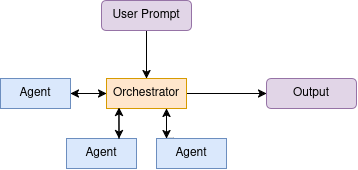
\includegraphics[width=1.0\textwidth]{figures/mas-centr.png}
		\caption{Three sub-agents are centrally controlled by an \emph{orchestrator}, which resolves
		conflicts, deduplicates information and arbitrates between worker agents.}
	  \end{figure}
	\end{column}
    \begin{column}{0.5\textwidth}
	  \begin{itemize}
		\item Also called ``hierarchical'' or ``layered'' systems
		\item Top-down control where a higher-level orchestrator makes
			decisions, manages and delegates tasks to sub-agents
		\item Naturally suited for tasks that are easily decomposable
	  \end{itemize}
	\end{column}
  \end{columns}
\end{frame}

\begin{frame}{Decentralized Multi-Agent Systems}
  \begin{columns}[T,onlytextwidth]
    \begin{column}{0.5\textwidth}
	  \begin{figure}
		\centering
		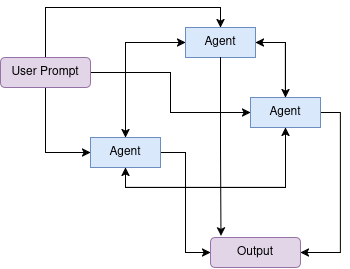
\includegraphics[width=1.0\textwidth]{figures/mas-decentr.png}
		\caption{Three agents are organized in a peer-to-peer network, occasionally synchronizing.}
	  \end{figure}
	\end{column}
    \begin{column}{0.5\textwidth}
	  \begin{itemize}
		\item Distribute decision-making across a network of (mostly) independent agents (peer-to-peer)
		\item Peer-to-peer removes centralized bottlenecks but makes synchronization expensive
		\item Also highly suited to decomposable tasks, but inter-agent synchronization constraints 
			must be relaxed to allow for somewhat infrequent output exchanges (e.g. debate scenario)
	  \end{itemize}
	\end{column}
  \end{columns}
\end{frame}

\section{Context Management}
\begin{frame}{Is Longer Context a Good Idea?}
  \begin{columns}[T,onlytextwidth]
    \begin{column}{0.5\textwidth}
	  \begin{figure}
		\centering
		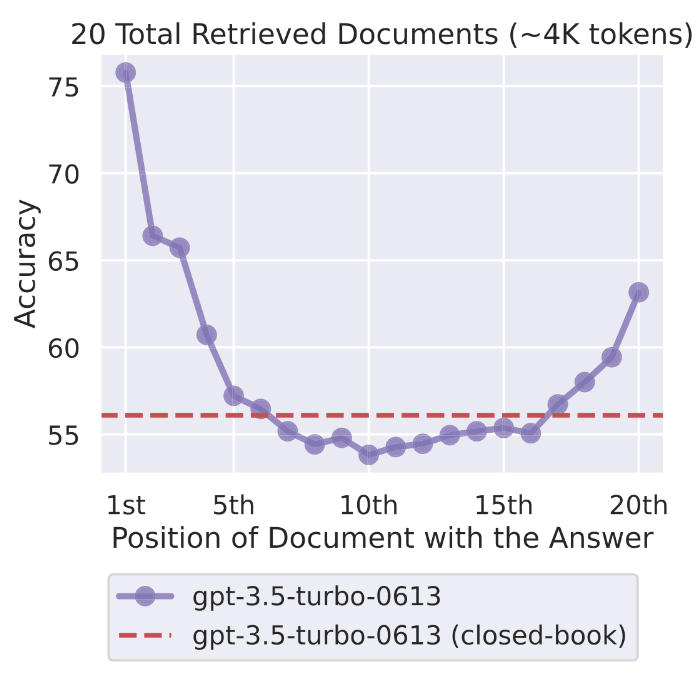
\includegraphics[width=0.9\textwidth]{figures/lost-middle.png}
		\caption{Longer context prevents agents from extracting necessary information 
		  that may be sandwiched in the middle
		  \href{direct.mit.edu/tacl/article/doi/10.1162/tacl_a_00638/119630/Lost-in-the-Middle-How-Language-Models-Use-Long}{(\underline{source})}.}
	  \end{figure}
	\end{column}
    \begin{column}{0.5\textwidth}
	  \begin{figure}
		\centering
		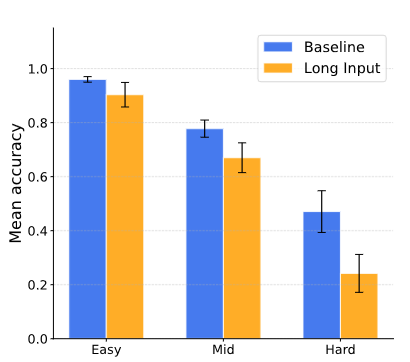
\includegraphics[width=0.9\textwidth]{figures/reason-shift.png}
		\caption{Irrelevant context build-up leads to accuracy drops and less self-verification
		  \href{arxiv.org/abs/2604.01161}{(\underline{source})}.}
	  \end{figure}
	\end{column}
  \end{columns}
\end{frame}

\begin{frame}{Managing Context in Multi-Agent Systems}
	\begin{itemize}
		\item Orchestrators in centralized multi-agent systems are often overwhelmed with context by
			sub-agents
		\item Passing only the minimal relevant context remains an issue
		\item Some papers propose using database-inspired transaction mechanisms and ``context repos''
			in order to reliably track context accumulation over time, and to prune out old context
		\item Another approach is to dynamically limit the amount of context an orchestrator
			receives, to focus its reasoning on a single sub-agent at a time
	\end{itemize}
\end{frame}

\section{Measuring and Evaluating Agents}

\begin{frame}{Accuracy is Not the Only Metric You Need}
	\begin{itemize}
		\item Benchmarks fail to do a holistic evaluation in AI agent capabilities, focusing mostly
			on accuracy scores
		\item Instead of pattern-matching, benchmarks often use LLM-as-judge to evaluate agent
			responses
		\item Cost, latency, efficacy, assurance and reliability are also important operational
			metrics
		\item Due to this discrepancy, agent systems tend to fail in real-world deployments
		\item Limited tracing practices prevents full introspection of agentic systems
	\end{itemize}
\end{frame}

\section{Discussion and Future Work}

\begin{frame}{Underexplored Aspects of Agent Systems}
	\begin{itemize}
		\item Context management remains a key issue that affects how an agent system solves a task
		\item Agent observability is lacking or limited, so complex interactions between agents are
			not fully understood
		\item Setting constraints on agent systems is a good solution, but these design decisions
			are informed by a thorough understanding of agent heuristics and biases
	\end{itemize}
\end{frame}

\section{Conclusion}
\begin{frame}{Summary}
	\begin{itemize}
		\item AI agents have shifted from being simple zero-shot interfaces to becoming autonomous
			systems that can attempt multi-step tasks with minimal human intervention
		\item However, these agents continue to lack reliability and optimal constraints that allow
			for bounded and more predictable behaviour
		\item This presentation showed the key architectural and orchestration strategies employed
			for single and multi-agent systems
		\item Context management and agent communication remain key challenges
		\item Better benchmarks and observability can help mitigate these issues
	\end{itemize}
\end{frame}

\begin{frame}[standout]
	Questions?
\end{frame}

\end{document}